\documentclass[border=5pt]{standalone}
\usepackage{tikz}
\usepackage{amsmath}
\usetikzlibrary{calc, positioning, arrows.meta, 3d}
\begin{document}
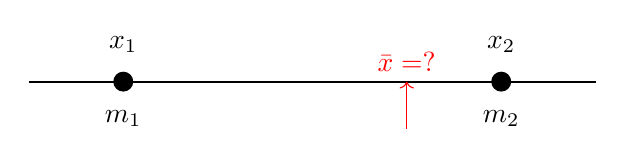
\begin{tikzpicture}[scale=1.2]
% Draw rod
\draw[thick] (0,0) -- (6,0);
% Mark masses
\fill (1,0) circle (3pt);
\node[below] at (1,-0.2) {$m_1$};
\node[above] at (1,0.2) {$x_1$};
\fill (5,0) circle (3pt);
\node[below] at (5,-0.2) {$m_2$};
\node[above] at (5,0.2) {$x_2$};
% Mark unknown center
\draw[red, ->] (4,-0.5) -- (4,0) node[above] {$\bar{x} = ?$};
\end{tikzpicture}
\end{document}
